\documentclass[10pt]{article}
\usepackage{enumitem}
\usepackage{hyperref}
\usepackage{float}
\usepackage{graphicx}

\title{Requirements Engineering\\SEM-Group 86}
\author{
	Ivar de Bruin\\
	4944135
	\and
	Tim Anema\\
	4953940
	\and
	Laura Pircalaboiu\\
	4777778
	\and
	Marc Otten\\
	4872541\\
	\and
	Ilya Grishkov\\
	4770811	
}

%forces a pagebreak before a new section
\let\oldsection\section
\renewcommand\section{\clearpage\oldsection}

\begin{document}
\maketitle
\pagebreak
\tableofcontents
\section{Requirement Engineering}
	\subsection{Functional requirements}
		\subsubsection{Must have}
			\begin{enumerate}
				\item The starting player must be chosen using a random number generator.
				\item There must be a GUI showing the current position of the balls on the table and the position of the cue stick.\label{req:GUITable}
				\item When aiming your shot, there must be a line indicating where the cue ball will go.
				\item There must be a menu showing scores. \label{req:scoreMenu}
				\item At the end of the game the score must be uploaded to the database with a name entered at that point.	\label{req:leaderboardName}
				\item There must be a way to play locally against other players.\label{req:localPlay}
				\item At the end of each game the top five scores ever should be shown.\label{req:leaderboardDisplay}
				\item The user must be able to register for an account.\label{req:register}
				\item The user must be able to authenticate.\label{req:login}
			\end{enumerate}

			\paragraph{Game Rules(8-ball)}
				\begin{enumerate}[resume]
					\item When the cue ball is potted, the other player must place it back in a place of his/her choosing.
					\item Each player must be assigned either stripes or solids.
					\item These types must be assigned based on the first ball potted after the break shot.
					\item When the first ball hit by a player is not his/her, it is counted as a foul and his/her turn ends and the other player may place the cue ball.\label{req:foulWrongBall}
					\item The black ball belongs to no player unless he/she has potted all of their assigned balls(striped or solid).\label{req:foulBlackBall}
					\item When the black ball is potted before all other balls belonging to that player are potted, said player will lose the game immediately.
					\item When a ball is potted it must be removed from the table.
					\item When the cue ball is potted it must instead be put back by the other player whose turn then starts.
				\end{enumerate}

			\paragraph{Collisions}
				\begin{enumerate}[resume]
					\item Collision between balls must be handled according to proper physics.\label{req:ballCollision}
					\item When a ball hits the wall it must bounce off correctly.
				\end{enumerate}

		\subsubsection{Should have}
			\begin{enumerate}[resume]
				\item There should be a settings page for graphical and sound settings.
				\item There should be statistics kept.
				\item There should be animations indicating the movement of balls.
				\item There should be sounds when collisions occur with balls, walls, pockets or cues.
				\item There should be an option to play online against another human player.
			\end{enumerate}

		\subsubsection{Could have}
			\begin{enumerate}[resume]
				\item A tutorial to explain the rules and controls to a new player could be implemented.
				\item There could be spin physics.
				\item There could be an option to chat with your opponent.
				\item There could be additional prediction lines after hitting the first ball.
				\item There could be camera controls.
			\end{enumerate}

			\paragraph{Other game types}
				\begin{enumerate}[resume]
					\item There could be an option to play against an AI.
					\item There could be an option to play 9-ball.
					\item There could be an option to play snooker.
				\end{enumerate}

		\subsubsection{Won't have}
			\begin{enumerate}[resume]
				\item We will not implement jump shots.
				\item We won't have micro-transactions.
			\end{enumerate}
	\pagebreak
	\subsection{Non-Functional requirements}
		\begin{enumerate}
			\item We need to use Java.
			\item Players must authenticate using a username and password.
			\item Players should be able to delete their data in compliance with GDPR.
			\item The application should run stable on the latest stable release of Windows 10, OS X and Linux (Manjaro and Arch Linux)
			\item The server container could be horizontally scaleable
		\end{enumerate}

		\subsubsection{Database}
			\begin{enumerate}[resume]
				\item A SQL database must be used to store scores and accounts.
				\item Interaction with the database must go through JDBC.
				\item JDBC's prepared statement must be used to prevent security vulnerabilities.
			\end{enumerate}

\section{Modelling use cases}
	\subsection{Logging in}
	\subsubsection{Description}
		\begin{itemize}
			\item{Use Case:} Logging in
			\item{Author:} Tim Anema
			\item{Date:} 28/11/2019
			\item{Purpose:} Authenticating with the server.
			\item{Overview:} Once the user opens the client, the client requests the user's credentials.
			Once the user has entered their credentials, the client will attempt to verify the user's credentials by contacting the server.
			If the verification is successful, the client will be able to start a game; otherwise (unsuccessful verification) a message is shown to the user.
			\item{Cross-reference:} Functional Requirement: \ref{req:login}
			\item{Actors:} User and server.
			\item{Pre-conditions:}
				\begin{itemize}
					\item The user must have opened the client.
					\item The user must have indicated he/she wants to login.
				\end{itemize}
			\item{Post-conditions:}
				\begin{itemize}
					\item A token was generated for use by the client
					\item A refresh token was generated for use by the client
				\end{itemize}
				\item{Flow of events:} See table below
			\end{itemize}
		\begin{figure}[H]
						\begin{tabular}{|p{45mm}|p{45mm}|p{45mm}}
User Actions                                  & System Action                                &
Server Action                                                              \\
\hline
1. User enters credentials& &  \\
& 2. Client sends credentials to server &  \\
& &   3. Server verifies credentials   \\
& &4. Server generates a token and a refresh token\\
& &5. Server sends token to client\\
& 6. Client stores token &   \\
7. User can continue.  & & \\
			\end{tabular}
		\end{figure}
		\subsubsection{UML Diagram}
			\begin{figure}[H]
				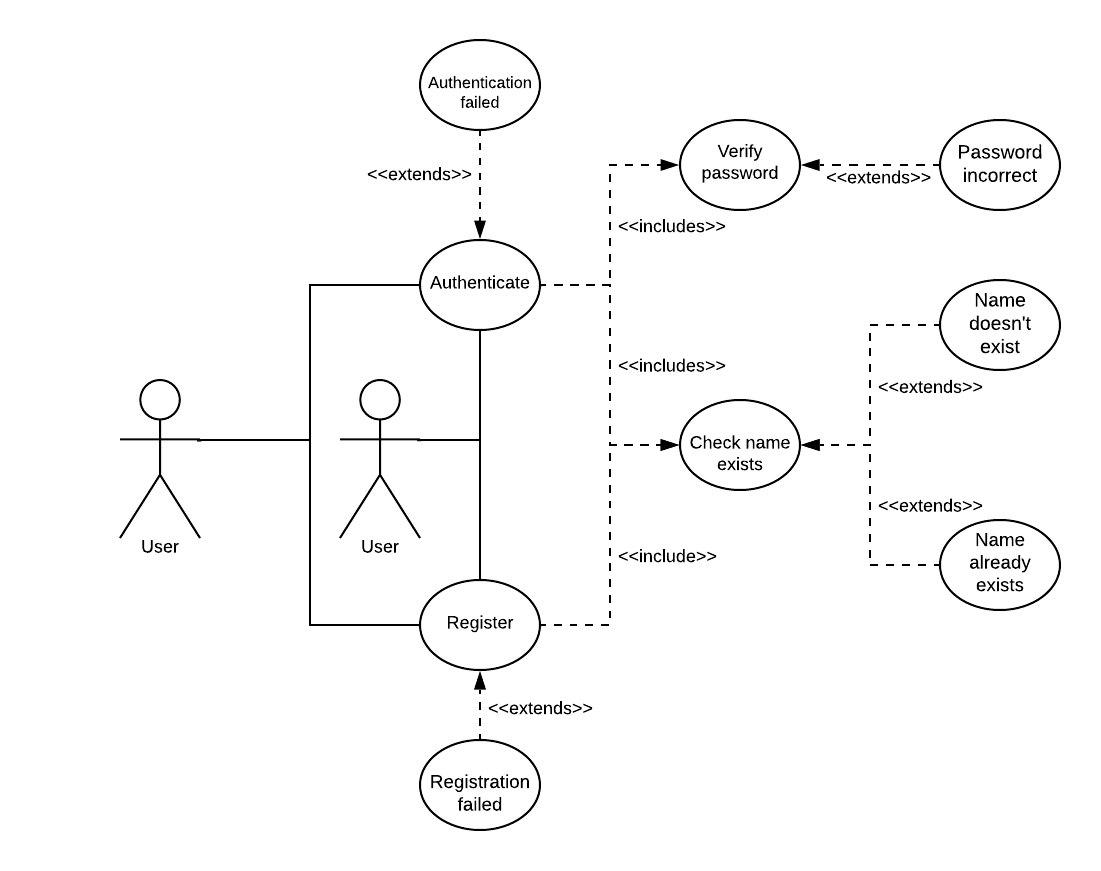
\includegraphics[width=1.1\linewidth]{latex_images/LoginAndRegisterUseCase.png}
				\caption{Logging in use case (upper use case)}
			\end{figure}
	\subsection{Registering a new player}
			\begin{itemize}
			\item{Use Case:} Registering
			\item{Author:} Tim Anema
			\item{Date:} 28/11/2019
			\item{Purpose:} Registering a new account.
			\item{Overview:} Once the user opens the client and indicates he/she wants to register a new account, the client asks for the required information (username and password).
			Once the user has entered the required information, the client will sends the information to the server. If the registration is succesful, the client will be able to login to their new account; otherwise (unsuccessful registration) a message is shown to the user.
			\item{Cross-reference:} Functional Requirement: \ref{req:register}
			\item{Actors:} User and server.
			\item{Pre-conditions:}
				\begin{itemize}
					\item The user must have opened the client.
					\item The user must have indicated he/she wants to register.
				\end{itemize}
			\item{Post-conditions:}
				\begin{itemize}
					\item A new user account should be saved in the database
				\end{itemize}
				\item{Flow of events:} See table below
			\end{itemize}
		\begin{figure}[H]
						\begin{tabular}{|p{45mm}|p{45mm}|p{45mm}}
User Actions                                  & System Action                                &
Server Action                                                              \\
\hline
1. User sends information & &  \\
& 2. Client sends information to server &  \\
& &   3. Server makes sure the name is not taken  \\
& &4. Server saves a new account in the database\\
& &5. Server sends a confirmation to client\\
6. User can continue  & & \\
			\end{tabular}
		\end{figure}
		\subsubsection{UML Diagram}
			\begin{figure}[H]
				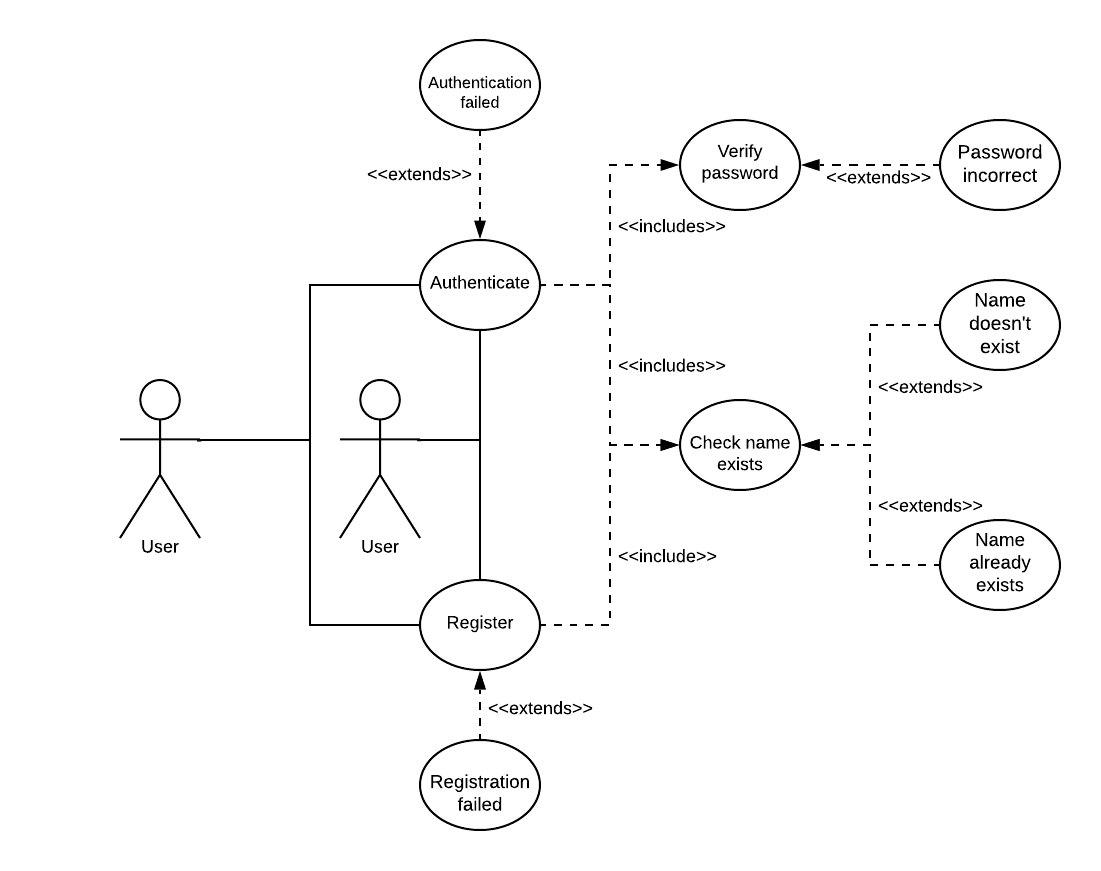
\includegraphics[width=1.1\linewidth]{latex_images/LoginAndRegisterUseCase.png}
				\caption{Registering use case (lower use case)}
			\end{figure}
	\subsection{Starting a game}
		\subsubsection{Description}
		\begin{itemize}
			\item{Use Case:} Starting the game.
			\item{Author:} Marc Otten.
			\item{Date:} 28/11/2019
			\item{Purpose:} Starting and setting up the game after user decides to start playing.
			\item{Overview:} After logging in and authenticating the user can start a game.
			When the user presses start game the game will be set up by the application using the proper
			rules and objects.
			\item{Cross-reference:} Functional Requirement: \ref{req:GUITable}, \ref{req:localPlay}
			\item{Actors:} Players.
			\item{Pre-conditions:} 
				\begin{itemize}
					\item The user must be logged in and use a valid session.
				\end{itemize}
			\item{Post-conditions:}
				\begin{itemize}
					\item The game must be started.
					\item The game must use the correct objects.
					\item The game must use the correct rules.
				\end{itemize}
				\item{Flow of events:} See table below
			\end{itemize}
		\begin{figure}[H]
			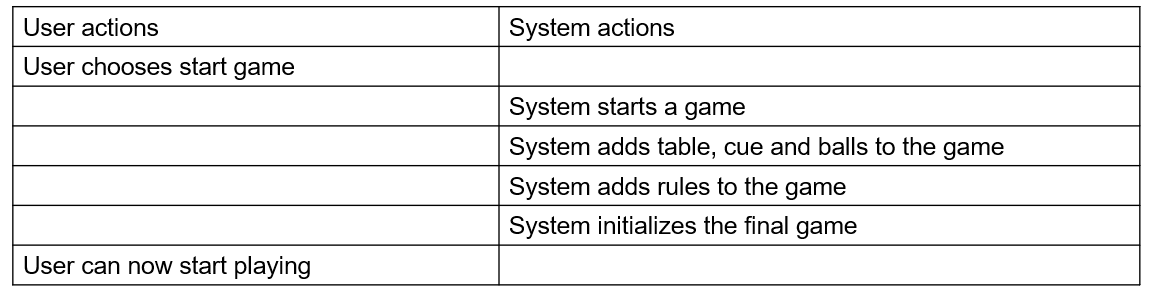
\includegraphics[width=\linewidth]{latex_images/StartgameTable.png}
			\caption{Table of event flow for starting a game.}
		\end{figure}
		\subsubsection{UML Diagram}
			\begin{figure}[H]
				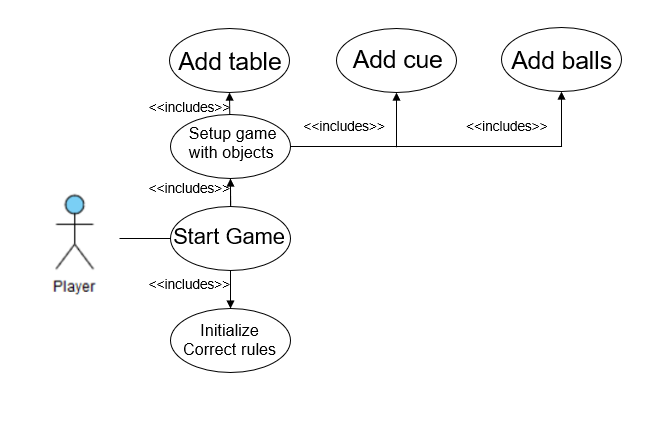
\includegraphics[width=\linewidth]{latex_images/StartgameUseCase.png}
				\caption{Starting a game use case diagram}
			\end{figure}
			
	\subsection{Hitting a ball}
		\subsubsection{Description}
		\begin{itemize}
			\item{Use Case:} A ball gets hit by a cue or another ball.
			\item{Author:} Marc Otten.
			\item{Date:} 28/11/2019
			\item{Purpose:} Handling physics and collisions correctly.
			\item{Overview:} When a ball gets hit by either a cue or another ball the collison gets handled correctly. This mean that it applies the physics rules we implemented and handles the collisions correctly. After the ball gets hit its momentum changes. It also checks on the first with the cue ball if the ball is of the correct type, if not it is considered a foul.
			\item{Cross-reference:} Functional Requirement: \ref{req:GUITable}, \ref{req:foulWrongBall}, \ref{req:foulBlackBall}, \ref{req:ballCollision}
			\item{Actors:} Players.
			\item{Pre-conditions} 
				\begin{itemize}
					\item The game must be started.
					\item It must be the player his/her turn.
				\end{itemize}
			\item{Post-conditions:}
				\begin{itemize}
					\item The ball must have the correct momentum.
				\end{itemize}
				\item{Flow of events:} See table below
			\end{itemize}
		\begin{figure}[H]
			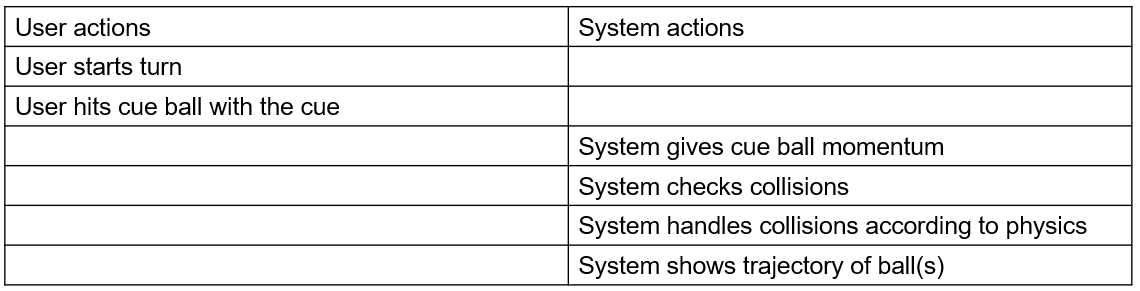
\includegraphics[width=\linewidth]{latex_images/HittingBallTable.png}
			\caption{Table for event flow of hitting a ball.}
		\end{figure}
		\begin{figure}[H]
			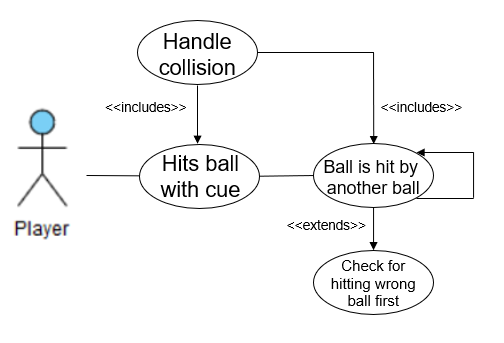
\includegraphics[width=\linewidth]{latex_images/HittingBallUseCase.png}
			\caption{Hitting a ball use case diagram}
		\end{figure}
		
	\subsection{Pocketing a ball}
	\subsubsection{Description}
		\begin{itemize}
			\item{Use Case:} Pocketing a ball.
			\item{Author:} Laura Pircalaboiu.
			\item{Date:} 28/11/2019
			\item{Purpose:} Pocketing a ball and deciding game flow afterwards.
			\item{Overview:} After a ball has been pocketed, a number of things can happen. If the ball is colored (i.e.: not the cue ball or the black ball), if it is the current player's color, then the current player will get an extra turn. If it is the opponent player's color, the opponent will get to place the cue ball wherever they want on the table.\\
			If the black ball has been pocketed after every other ball, the current player wins. Otherwise, the current player instantly loses.
			If the cue ball has been pocketed, the opposing player can get to place the cue ball wherever they want.
			\item{Cross-reference:} Functional Requirement: \ref{req:foulWrongBall}, \ref{req:foulBlackBall}, \ref{req:ballCollision}
			\item{Actors:} Balls.
			\item{Pre-conditions} 
				\begin{itemize}
					\item The game must have been completed.
					\item The user must be in a valid session.
				\end{itemize}
			\item{Post-conditions:}
				\begin{itemize}
					\item The game must proceed based on the penalties or bonuses decided.
					\item If the black ball has been pocketed, the game must end.
				\end{itemize}
			\item{Flow of events:} See table \ref{eventFlow:pocketBall}
		\end{itemize}
		\begin{table}[H]
		\label{eventFlow:pocketBall} 
			\begin{tabular}{|p{45mm}|p{45mm}|p{45mm}}
User Actions                                  & System Action                                & 
Server Action                                                              \\
\hline
1. Ball collides with another ball& 2. System updates ball locations           &                                                                            \\
                    3. Ball gets pocketed & &                                       \\
                                              &    4. System checks color of ball and decides flow of events &  \\
                                              & 5. System sends updated game state to user. &                                                                            \\6. User can see the updated game state.                &                                              &                                                                           
			\end{tabular}
		\caption{Flow of events of use case \ref{useCase:leaderboard}}
		\end{table}
		\subsubsection{UML Diagram}
		\begin{figure}[H]
			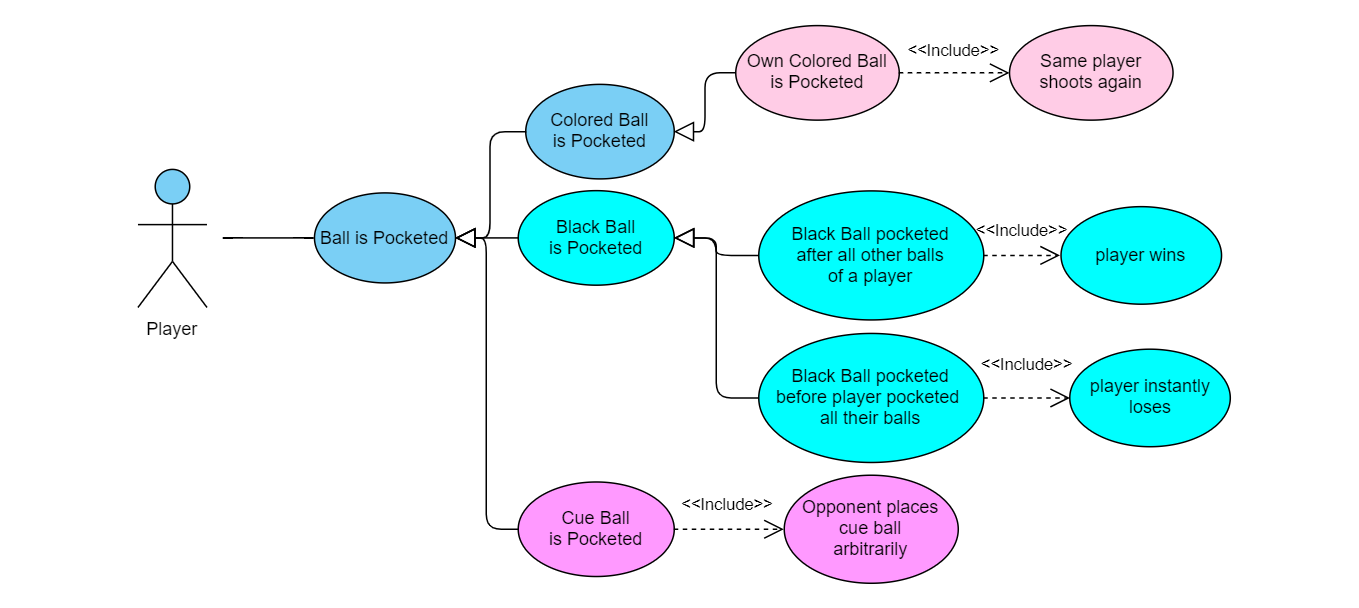
\includegraphics[width=\linewidth]{latex_images/pocketing_ball.png}
			\caption{Pocketing a ball use case diagram}
		\end{figure}
		
	\subsection{Updating the leaderboard}\label{useCase:leaderboard}
		\subsubsection{Description}
		\begin{itemize}
			\item{Use Case:} Updating the leaderboard.
			\item{Author:} Ivar de Bruin.
			\item{Date:} 28/11/2019
			\item{Purpose:} Adding an achieved score to the leaderboard and displaying it to the user.
			\item{Overview:} After a game a player can update the name that will be shown along with his achieved score for that game on the leaderboard. This score will be send to the server.
			The server will add it to the database linked to the correct user.
			The server will then send back the updated leaderboard to the user.
			\item{Cross-reference:} Functional Requirement: \ref{req:scoreMenu}, \ref{req:leaderboardName}, \ref{req:leaderboardDisplay}
			\item{Actors:} Players and Server.
			\item{Pre-conditions} 
				\begin{itemize}
					\item The game must have been completed.
					\item The user must be in a valid session.
				\end{itemize}
			\item{Post-conditions:}
				\begin{itemize}
					\item The score must be stored in the database linked to the user account.
					\item The leaderboard must be updated to show the new top 5 scores ever.
					\item The name chosen by the user must be stored so entering it again is unnecessary.
				\end{itemize}
			\item{Flow of events:} See table \ref{eventFlow:leaderboard}
		\end{itemize}
		\begin{table}[H]
		\label{eventFlow:leaderboard} 
			\begin{tabular}{|p{45mm}|p{45mm}|p{45mm}}
User Actions                                  & System Action                                & 
Server Action                                                              \\
\hline
1. User updates leaderboard name if necessary & 2. System updates leaderboard name           &                                                                            \\
                                              & 3. System sends score to the server          & 4. Server adds score to the database                                       \\
                                              &                                              & 5. Server creates new leaderboard consisting of top 5 scores ever achieved \\
                                              & 6. System sends updated leaderboard to user. &                                                                            \\
7. User views the leaderboard.                &                                              &                                                                           
			\end{tabular}
		\caption{Flow of events of use case \ref{useCase:leaderboard}}
		\end{table}
		\subsubsection{UML Diagram}
		\begin{figure}[H]
			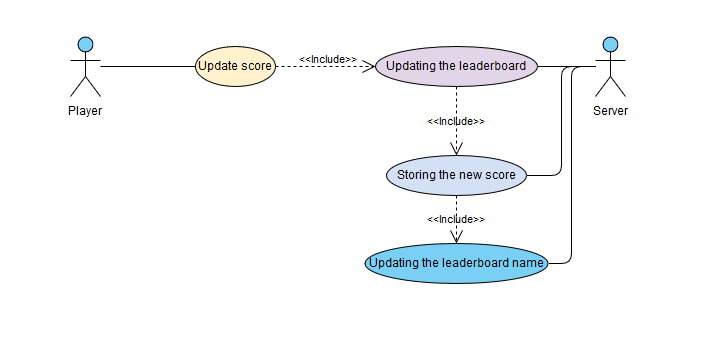
\includegraphics[width=\linewidth]{latex_images/LeaderboardUseCase.png}
			\caption{Adding a score to the leaderboard use case diagram}
		\end{figure}
\end{document}